\documentclass[10pt]{article}
\usepackage[spanish]{babel}
\usepackage[margin=1.6cm]{geometry}
\usepackage{amsmath,graphicx}

\title{Espaciamientos a primeros vecinos:\\ distribución exacta contra Wigner surmise}
\author{Carlos Pineda}
\date{12 de octubre de 2026}\vspace{-1em}

\begin{document}
\maketitle

\section{Pregunta}

La distribución de espaciamientos a primeros vecinos, $P(s)$, de los ensambles
gaussianos suele compararse con el Wigner surmise,
\begin{equation}
  P_1(s) = \frac{\pi s}{2}\, e^{-\pi s^2/4}, \qquad
  P_2(s) = \frac{32 s^2}{\pi^2}\, e^{-4 s^2/\pi},
\end{equation}
que es exacto para matrices de $2\times2$. Para $N\to\infty$, la distribución
exacta es distinta, pero la diferencia es pequeña: alrededor de 1\%. En
\texttt{TheoreticalRMT.m}, la función \texttt{P[s,$\beta$]} da el surmise y
\texttt{ExactPs[$\beta$,s]} da la distribución exacta. Esta última interpola
(orden 3) las tablas de Mehta y Haake, con $0\le s\le 3.69$. Quisimos saber si
una simulación numérica distingue las dos curvas y si sigue a la exacta.

\section{Qué se hizo}

\paragraph{Matrices.} Para GOE ($\beta=1$) tomamos $H=(A+A^T)/2$, con
$A_{ij}$ reales e independientes, $A_{ij}\sim\mathcal N(0,1)$. Para GUE
($\beta=2$) tomamos $H=(A+A^\dagger)/2$, con $A_{ij}$ complejos y
$\langle|A_{ij}|^2\rangle=1$. En ambos casos
$\langle|H_{ij}|^2\rangle=1/2$ fuera de la diagonal, así que la densidad es un
semicírculo de radio $R=\sqrt{2N}$. Usamos $N=200$ y $2\times10^5$ matrices
por ensamble.

\paragraph{Despliegue.} Cada autovalor $x$ se transforma con la función de
conteo del semicírculo,
\begin{equation}
  \mathcal N(x) = N\left[\frac12 + \frac{x\sqrt{R^2-x^2}}{\pi R^2}
    + \frac1\pi \arcsin\frac{x}{R}\right],
\end{equation}
y solo se usa la mitad central del espectro, para evitar los bordes. Así
obtenemos $2\times10^7$ espaciamientos por ensamble. La corrida tarda unos
2,5 minutos en 64 núcleos.

\paragraph{Comparación.} Usamos bins de ancho $w=0.1$. Si un bin tiene $c$
cuentas de un total de $M$, su densidad es $c/(Mw)$, con error
$\sqrt c/(Mw)$ (Poisson). A cada bin le restamos el promedio de $P(s)$ sobre
el bin, no su valor en el centro. Así evitamos un sesgo por curvatura de orden
$w^2P''/24\approx10^{-3}$, comparable a la señal.

\begin{figure}[!htb]
  \centering
  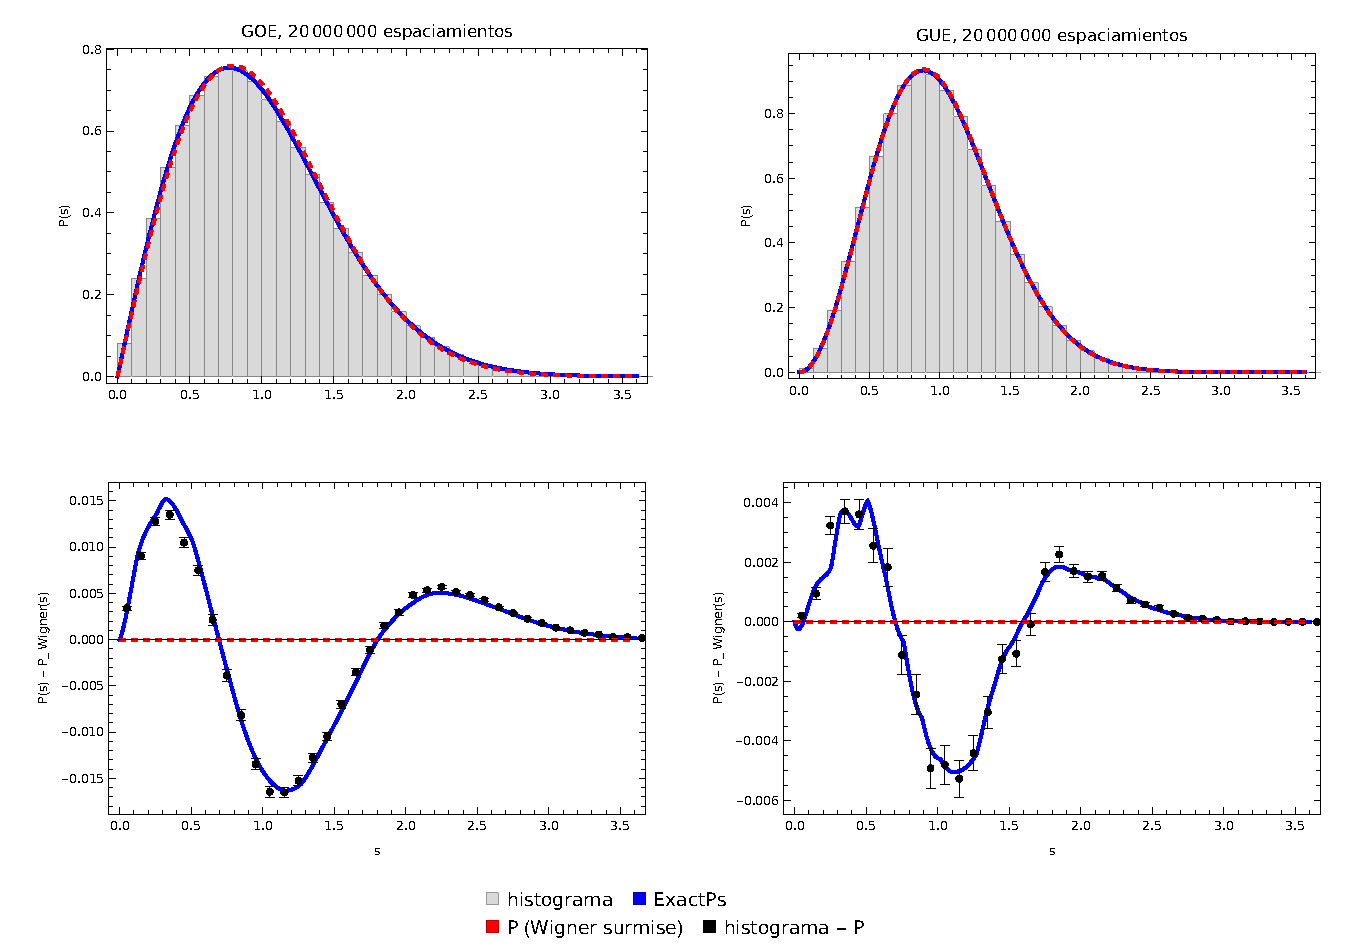
\includegraphics[width=0.68\textwidth]{fig_nns.pdf}
  \caption{Arriba: histograma de espaciamientos, \texttt{ExactPs} (azul) y
    Wigner surmise (rojo). Abajo: histograma menos el surmise (puntos) y
    \texttt{ExactPs} menos el surmise (azul). Izquierda GOE, derecha GUE;
    $N=200$, $2\times10^7$ espaciamientos por ensamble.}
  \label{fig:nns}
\end{figure}

\section{Resultado}

En el histograma (figura~\ref{fig:nns}, arriba) las dos curvas casi no se
distinguen. La diferencia (abajo) sí las separa. En GOE, la distribución
exacta se aparta del surmise en $\pm0.015$, con un máximo en $s\approx0.3$ y un
mínimo en $s\approx1.1$. El error por bin es de unos $3\times10^{-4}$, así
que la simulación descarta el surmise por unas 50 desviaciones estándar y
reproduce la forma de \texttt{ExactPs}$-P$. En GUE la diferencia es tres
veces menor, $\pm0.005$, y los datos también la siguen.

\section{El pequeño desajuste en GOE}

En GOE los datos quedan algo por debajo de \texttt{ExactPs} cerca del máximo
de la diferencia ($s\approx0.3$--$0.5$, unos $1.5\times10^{-3}$) y algo por
encima en la cola ($s\approx2.2$, unos $7\times10^{-4}$). Son varias
desviaciones estándar, y el patrón se repite en corridas independientes, así
que no es ruido. Consideramos tres causas.

\paragraph{1. Escala del despliegue (la principal).} El espaciamiento medio
debería ser 1. En GUE obtenemos $\langle s\rangle=1.0000$, pero en GOE
$\langle s\rangle=1.0013$. Si todos los espaciamientos están estirados por un
factor $1+\varepsilon$, la distribución observada es
\begin{equation}
  P_{\rm obs}(s)=\frac{1}{1+\varepsilon}P\!\left(\frac{s}{1+\varepsilon}\right)
  \approx P(s)-\varepsilon\,\big[P(s)+sP'(s)\big].
\end{equation}
Con $\varepsilon=0.0013$ esto predice $-1.1\times10^{-3}$ en $s\approx0.3$ y
$+5\times10^{-4}$ en $s\approx2.2$: el mismo signo y casi el mismo tamaño que
el desajuste. Para probarlo, reescalamos $s\to s/\langle s\rangle$ y
comparamos con \texttt{ExactPs} en 36 bins. El $\chi^2$ baja de 152 a 29, lo
que corresponde a puro ruido estadístico. El desajuste, por tanto, viene casi
todo de la escala.

\emph{Hipótesis (no comprobada):} el semicírculo es la densidad para
$N\to\infty$. Para GOE, la densidad a $N$ finito tiene correcciones de orden
$1/N$; para GUE empiezan en orden $1/N^2$. Eso explicaría por qué el error de
escala aparece en GOE y no en GUE. Repetir con $N=400$ debería reducirlo a la
mitad.

\paragraph{2. Tamaño finito más allá de la escala.} Aun bien desplegada, la
$P(s)$ de una matriz de $N=200$ no es exactamente el límite $N\to\infty$.
Después de reescalar, lo que queda es compatible con ruido, así que este efecto
es menor que $\sim3\times10^{-4}$ con esta estadística.

\paragraph{3. La tabla de \texttt{ExactPs}.} La tabla tiene 5 decimales y
está bien normalizada: $\int P\,ds$ y $\langle s\rangle$ valen 1 a
$10^{-4}$. Su interpolación cúbica sí deja artefactos visibles en GUE:
ondulaciones en $s\approx0.3$--$0.5$, donde el paso de la malla cambia en
$s=0.637$, y un valor negativo minúsculo ($-2.5\times10^{-5}$) cerca de
$s=0$. Estos artefactos no explican el desajuste de GOE. Para eliminarlos,
se podría calcular $P(s)$ con el determinante de Fredholm del kernel seno
(método de Bornemann), con precisión de $10^{-10}$.

Nota: los errores de Poisson ignoran las correlaciones entre espaciamientos
de un mismo espectro; podrían estar algo subestimados.

\section{Conclusión}

La simulación distingue con claridad la distribución exacta del Wigner surmise
y sigue a \texttt{ExactPs} en GOE y GUE. El único desajuste visible, en GOE,
viene de que el despliegue con el semicírculo da un espaciamiento medio
0,13\,\% mayor que 1; al corregir esa escala, los datos coinciden con
\texttt{ExactPs} dentro del ruido.

\textbf{Archivos.} \texttt{nns.nb} reproduce la figura (con
\texttt{reals = 20000} tarda unos 35\,s; la figura usa \texttt{reals =
200000}). \texttt{nns.wl} contiene el mismo código como script.

\end{document}
